\chapter{Predicting Stocks Using Sentiment Analysis - Felix} \label{ch:predictions_ml}
The movement of time series data for financial data is influenced by external effects. To leverage this we tried to add information from news sources to our trading strategies. For the hybrid prediction we estimate sentiment scores on news sources. This so called sentiment analysis is used to explore the orientation of the words or phrases in text data and their effect on the overall sentiment \citep{HADDI201326}. The original aim was to use financial news data to predict stock price movement and volatility for trading strategies. To achieve this, large amounts of text data would need to be preprocessed and analyzed regarding their connections to specific stocks, their topic and sentiment. The news data would need to be as precise as possible, because […] mention that an effect on the stocks an only be measured up to 20min after the news appear. Other sources say that… .
\\ \\
As we were not able to acquire access to a reliable and precise news sources, we tried to implement our approach on the available analyst reports regarding the ten specific stocks. The problem with these reports is, that they are more an indicator of performance over the past month and a prediction about the future performance. As such they do not cover sudden events that would be present in the news. The reports also cluster around certain dates with long stretches of no or very few reports in between (ABBILDUNG). This makes it unlikely that they are valuable for trading strategies.
%\begin{figure}[h]
%    \figuretitle{Seasonality in the Reports}
%    \centering
%    \begin{adjustbox}{width=.9\textwidth,center}
%    \input{figures/SeasonalityReports.png}
%    \end{adjustbox}  
 %   \caption{BLBLBLA}
 %   \label{fig:Seasonality in the Reports}
%\end{figure}{}
\\  \\
The goal was to identify the connection of specific articles to listed companies and compute a sentiment score for the article. There are many ways to calculate sentiment scores from flowing text data. Common procedures would be to use a library of previously known positive and negative adjectives or 4-grams. The simplest way to utilize these would be to simply count their appearance, this is known as a bag-of-words method (ZITAT?). Other approaches extract parts of the text at the location of the specific adjectives and use Support Vector Machines or Naive Bayes Classifier to extract sentiment, see \citet{westerski2007sentiment} for further references. Many of these more advanced sentiment classification techniques are supervised, as such the need a labelled data set for initial training. The (NUMBER \#) analyst reports are unstructured and not labelled making it unrealistic to use these methods. They also have a very specific format and language, therefore other pretrained models or other labelled training data sets could not be used. Another possibility to custom label the data would have been possible using intra day trading and news data. By looking at the movement or volatility of the period close after the news release approximate sentiment scores can then be computed \citep{robertson2007news}. As the obtained stock data is only inter day we could not apply this method.
\\ \\
Two methods to estimate sentiment scores in an unsupervised way will be explored here. One is a library bag-of-words approach that works with simple relative frequencies of positive and negative words. The other approach uses a new method called Joint Sentiment Topic model (JST) \citep{lin2009joint} and relies on a Bayesian method called Latent Dirichilet Allocation (LDA)  \citep{blei2003latent}. For both approaches the text data has to be cleaned which is described in section \ref{cleaningText}, the subsequent analysis of the sentiment scores can be found in section \ref{BoW} and \ref{JST}.

\subsection{Cleaning of the text data}\label{cleaningText}
To get reliable sentiment scores text data has to be preprocessed. WHY IMPORTANT READ: dimensionality of the problem, 157380 individual words and characters,  specially important for unsupervied approaches \citep{HADDI201326}. The preprocessing was done in five steps using \texttt{R} \citep{Rproject}. At first words where converted to lowercase and all words where separated using the R package \textit{tidytext} \citep{tidytext}. Next all the stop words where removed using the stop word library from the \textit{tidytext} package, as well as a custom set. This reduces the total number of words from 67M initially to 36M, see figure \ref{fig:TotWord}. In the next step all links to websites, hyper-references, numbers, words with numbers and punctuation are removed as well. Underlying the reduction in total number of words about 74320 individual special characters items are removed. 

%The analyst reports consist of scrapped text from reports that does nut necessarily follow a normal sentence like structure. This makes it difficult to apply syntactic based methods to extract adjectives from the flowing text based on semantic rules. 
\begin{figure}[h]
\centering
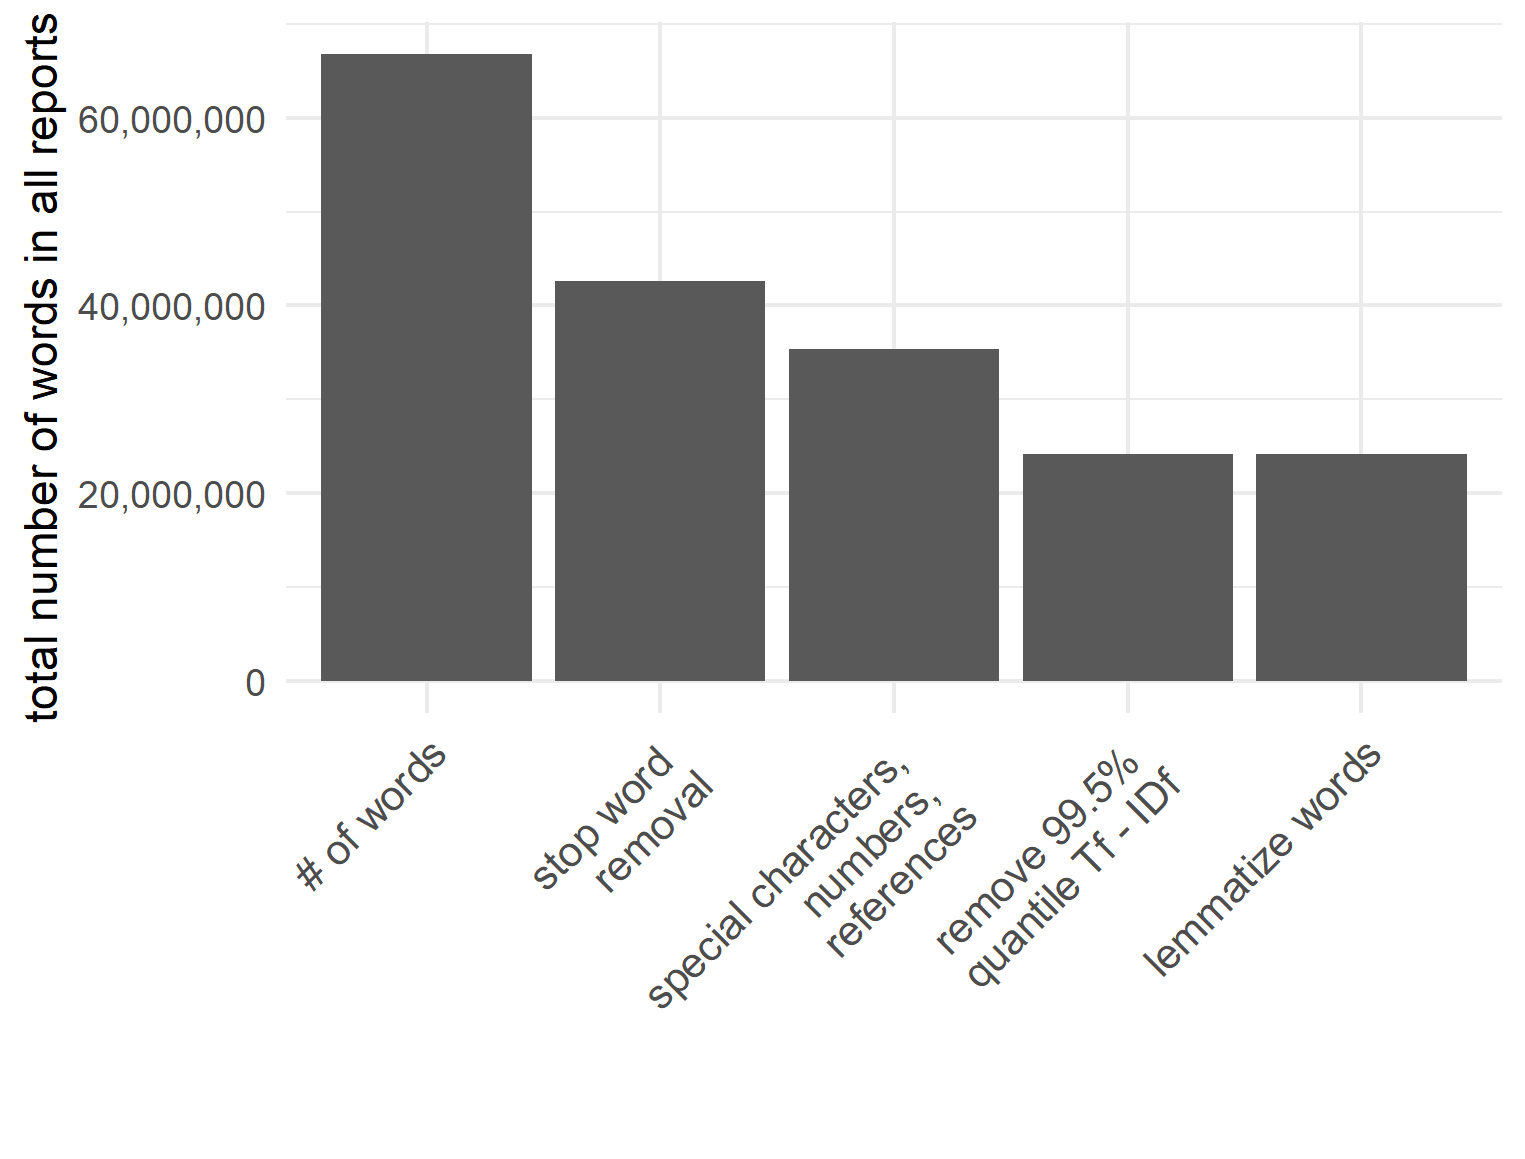
\includegraphics[width=\textwidth]{figures/ReductionInTotalNWords.png}
\caption{Reduction in total number of words due to preprocessing the data.}
\label{fig:TotWord}
\end{figure}

A common way to look at feature importance in flowing text data is to look at the Term Frequency Inverse Document Frequency (TF-IDF) which puts the feature frequency (FF) also called term frequency (TF) in relation to the inverse document frequency (IDF) \citep{na2004effectiveness}. 
\begin{equation}
    TF-IDF = FF * Log(\frac{N}{DF})
\end{equation} 
Where N represents the number of documents and is DF the number of documents that contain this feature, calculated as the sum of the feature presence (FP). The result is a probability between 0 and 1 for each word. For a large number of words s in our case TF-IDF values are usually quite low. To reduce the dimension of the data even further the 15 Percent of lowest scoring values was removed on the document level, leaving just over 34M words in total. This represents the removal of an additional 3502 individual words. The fifth and last step is lemmatizing the words using the \textit{textstem} package \citep{textstem}. Lemmatizing words means reducing them to their inflectional forms. Commonly stemming is also applied, because words sometimes have derivationally related forms. This was not done to have more flexibility for the later applied text analysis. \\ \\

After these five cleaning steps the number of individual words and items was reduced from 157380 to 70272 by about 44 Percent and of the total number of words only 5 Percent are left. The summary statistics for the total number of words in each report in table \ref{tab:summaryCR} show the result more clearly. 
\begin{table}[ht]
\centering
\begin{tabular}{rllllll}
  \hline
  & Min. & 1st Qu. & Median  &  Mean & 3rd Qu. &   Max. \\
  \hline
  original reports & 3    &  1907 &  3226  &  3827 &  4780 &  21502  \\ 
  cleaned reports  & 1  &  83 &  145 & 190.6 & 242.8 & 1747  \\ 
   \hline
\end{tabular}\label{tab:summaryCR}
\caption{Summary statistics for the number of words in each report}
\end{table}

After validating the cleaned text different uncleaned items, like woks consisting of multiples of the same letter, where discovered. We did not find a way to remove them.

\subsection{Sentiment Library}\label{BoW}
The simplest approach for estimating unsupervised sentiment scores is applying a library of as positive and negative words to the data. The resulting polarity towards positive or negative sentiment can then be achieved by simple relative probabilities
\begin{equation}
    Polarity = \frac{P - N}{P + N}
\end{equation}
of the sum of positive words (P) and negative words (N). 

cite specific sentiment library for analysis.
% latex table generated in R 3.6.0 by xtable 1.8-4 package
% Sun Sep 08 17:25:29 2019
\begin{table}[ht]
\centering
\begin{tabular}{rll}
  \hline
 & positive & negative \\ 
 & $n = 218$ & $n = 1282$ \\ 
  \hline
  1 & acclaim & abandonment \\ 
  2 & accomplishment & abdication \\ 
  3 & advantage & abuse \\ 
  4 & assure & acquittal \\ 
  5 & attractiveness & catastrophe \\ 
  6 & delightful & criticize \\ 
  7 & diligent & degrade \\ 
  8 & impress & harsh \\ 
  9 & \vdots & \vdots \\ 
   \hline
\end{tabular}
\end{table}
These results can be used to benchmark the results of the more advanced method.
\begin{figure}[h]
\centering
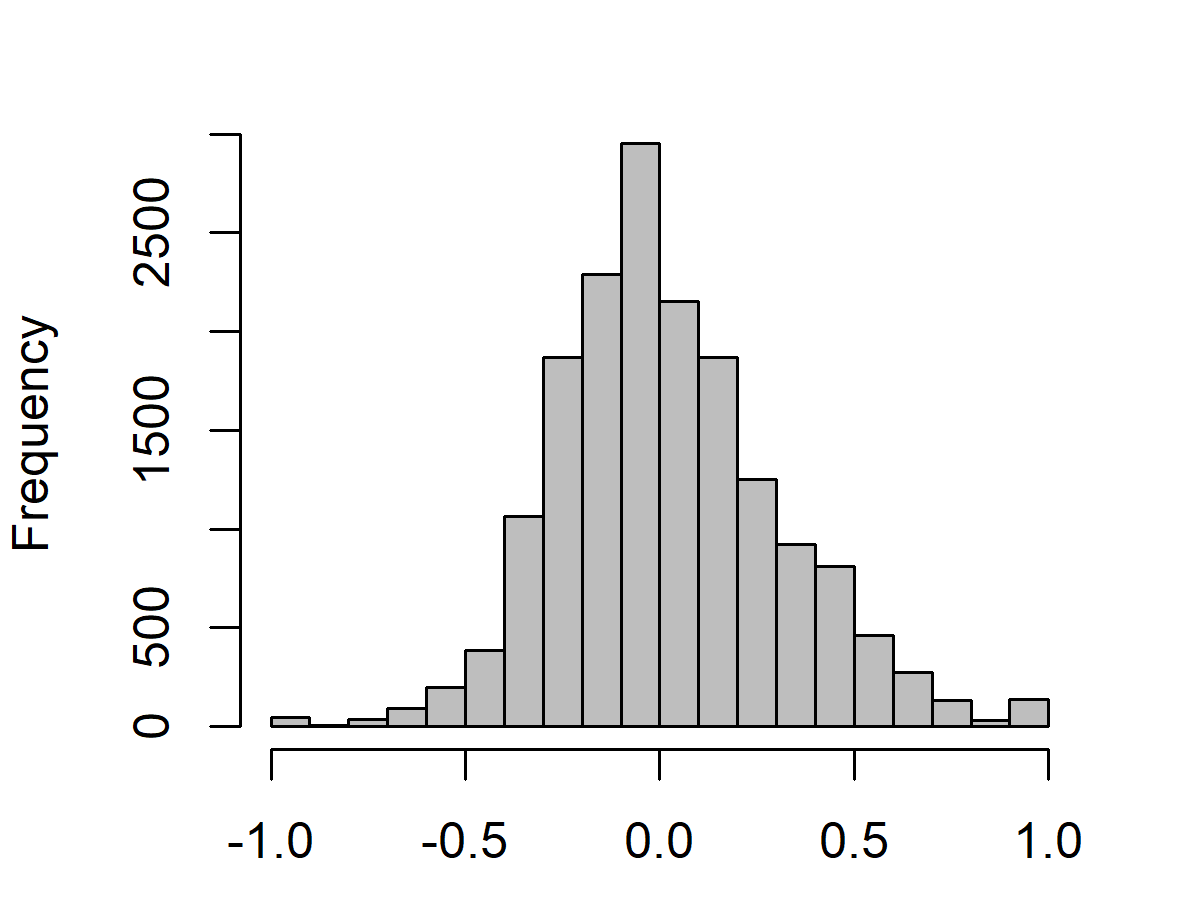
\includegraphics[width=\textwidth]{figures/2SentimentsBOW_Histogram.png}
\caption{Histogram of the sentiment scores computed by the sentiment library}
\label{fig:BoWSentiment}
\end{figure}



\subsection{Joint sentiment topic model}\label{JST}
To make the computation of the sentiment scores more adaptable to the specific format of the data a new method by \citet{lin2009joint} called Joint Sentiment Topic model (JST) for sentiment analysis is being used. This approach builds upon the idea of \citet{blei2003latent} to use a Bayesian hierarchical model, Latent Dirichilet Allocation (LDA), to compute topics from text data. Latend Dirichilet Allocation is one of the most sophisticated methods in the field of topic modelling. To understand JST we firstly explain the fundamentals and assumptions of LDA. \\ 

% good video: https://www.youtube.com/watch?v=DWJYZq_fQ2A
The general idea of LDA is that each document can be described by a distribution of topics and each topic can itself be described by a distribution of words \citep{blei2003latent}. This assumes that the words themselves are independent of each other which is in reality not the case but for large data sets this assumption seems to be acceptable. To train a LDA one decides on the number of topics ($T$) that occur within the text documents, but these topics have not been observed, they are latent. The LDA has two dirichilet priors containing hyperparameters $\alpha$ and $\beta$, a high $\alpha$ indicates that each document is likely to contain a mixture of many topics, similarly a high $\beta$ indicates that each topic is a mixture of many different words. LDA backtracks from the document level to identify topics that are likely to have generated this specific corpus of words. The underlying optimisation of the model is done using a Gibbs-Sampler. In the first step each word is assigned probabilities to belong to each of the $T$ topics that sum up to one and each document gets a probability for each topic. The algorithm then iterates over the words topics and documents, updating the underlying probabilities. \\ \\
In the JST the LDA is extended from three hierarchical layers to four. The additional layer models the document sentiment by adding a layer in between the document and topic layer \citep{lin2009joint}. The new sentiment layer can be associated with documents, followed by topics and then words. For a detailed mathematical definition see \citet{lin2009joint}. \\ \\
To estimate the JST models we used the \textit{rJST} package in R \citep{rJST}. The output are posterior probabilities for sentiments and topics of each document, as well as the posterior probabilities of each word loading onto topics. 

\textit{initial prior information by sentiment dictionary}

EVALUATION of results: The results of the JST model need to be evaluated if the results split the data in reasonable topics and how the distributions of the sentiment scores look. After computing JST models with 10, 20, 30 and 50 topics we decided that the model with 30 topics yields the best results. An overview over the first 15 words for topic one, two, three and thirty can be found in \ref{tab:TopicWordsSent1}. 

JST AND NEW DATA: For a large and diverse enough training data set the returned posterior probabilities of the words can be used to determine the topics and sentiment in new documents. The JST therefore does not need to be retrained at each new observation. 

% latex table generated in R 3.6.0 by xtable 1.8-4 package
% Wed Sep 11 23:03:36 2019
\begin{table}[ht]
\centering
\begin{tabular}{rllll}
  \hline
 & topic1sent1 & topic2sent1 & topic3sent1 & topic30sent1 \\ 
  \hline
1 & buckresearchcom & guggenheim & appointment & macquarie \\ 
  2 & buckingham & hotel & university & russell \\ 
  3 & hochstim & wunderlich & reinvest & thai \\ 
  4 & joseph & room & buysellsignals & mainland \\ 
  5 & amexs & monitor & retire & organisation \\ 
  6 & amex & morris & appoint & bandra \\ 
  7 & attain & suspension & chair & alliance \\ 
  8 & accumulate & disclosuresaction & council & file \\ 
  9 & christopher & weekend & board & amendment \\ 
  10 & retransmit & predictability & career & utility \\ 
  11 & brad & wknd & elect & remind \\ 
  12 & wilson & serv & relation & commonwealth \\ 
  13 & master & madison & bite & refrain \\ 
  14 & apparel & exploration & mcap & kasikorn \\ 
  15 & kevin & desk & oversee & endorse \\ 
   \hline
\end{tabular}\label{tab:TopicWordsSent1}
\end{table}

\begin{figure}[h]
\centering
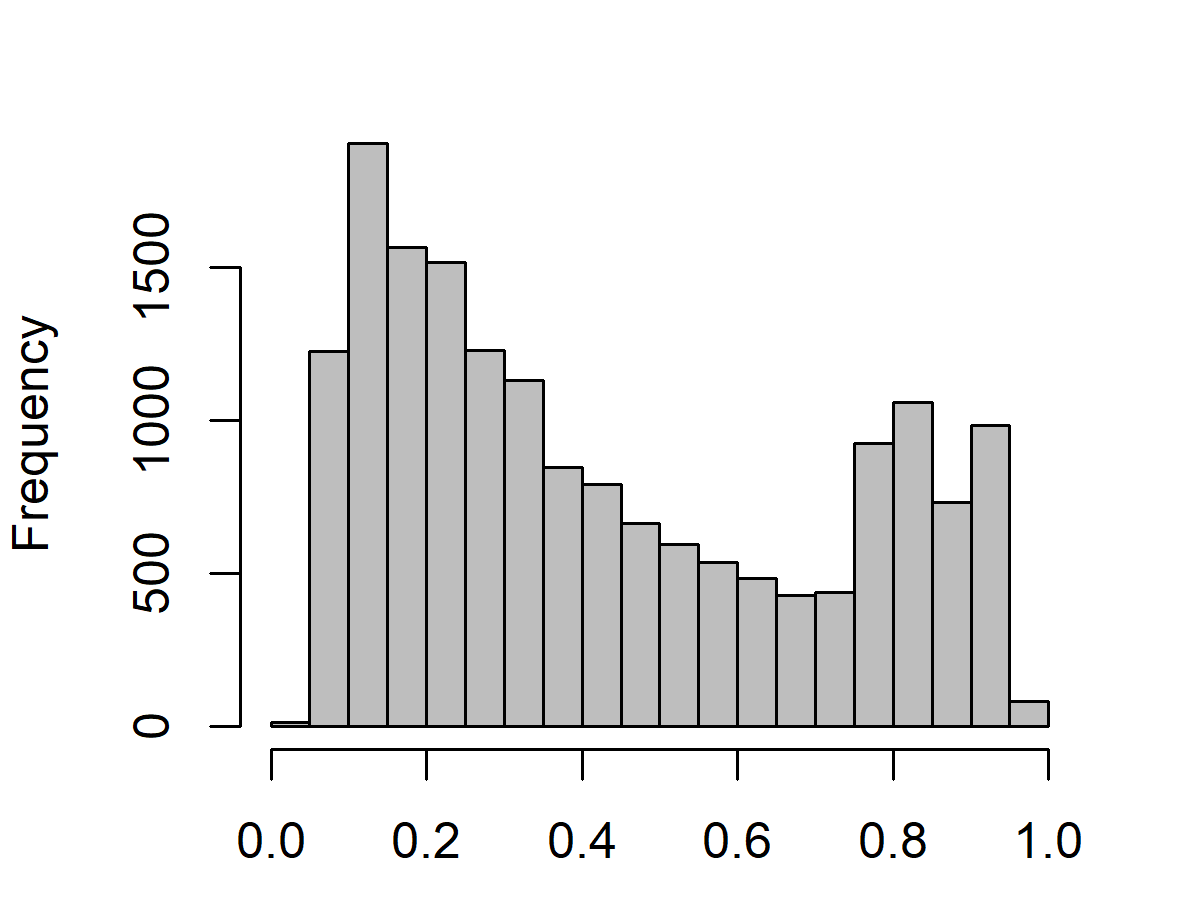
\includegraphics[width=4in]{figures/2SentimentsJST_Histogram.png}
\caption{Histogram of the sentiment scores computed by the Joined Sentiment Topic model}
\label{fig:JSTSentiment}
\end{figure}

\begin{enumerate}
    \item Weil wir nur wenige stocks haben kann es sein das das JST company specifix topics bildet
    \item Schätzen von neuen texten möglich basierend auf den posterior wort probabilities
    \item Histogram of sentiment
\end{enumerate}




\subsection{XG-Boost on sentiment data}
\begin{itemize}
    \item XGB kann auch einfach nur verwendet werden um zu erkennen welche features wichtig sind
\end{itemize}
\subsubsection{XGBoost}
Here I expalain what XGBoost is an how it works

\subsection{Classification results}
Take Mean of different predictions?

XGBOOST, LightGBM whatever. 
Theorie, Datenaufbereitung, Ergebnisse

The standard evaluation of binary classification results is done using the F1-measure \citep{HADDI201326}. Where the score is a weighted product of precision and recall
\begin{equation} 
    F-measure = \frac{2*precision * recall}{precision + recall}
\end{equation}

% https://www.kaggle.com/furiousx7/xgboost-time-series
% related literature at the end
% Hourly forecasting: https://www.kaggle.com/robikscube/tutorial-time-series-forecasting-with-xgboost/notebook
% https://www.datacamp.com/community/tutorials/xgboost-in-python
% missing values in XGB https://github.com/dmlc/xgboost/issues/21


